% =============================================================================
% Versao condensada para a Revista da Sociedade Brasileira de Medicina Tropical,
% Artigo Original: 3.500 palavras de texto, resumo de 250, 5 ilustracoes.
%
% O manuscrito completo continua em manuscript.tex e nao deve ser apagado: e o
% registro integral do trabalho, e a origem do material suplementar.
% Tabelas e figuras vem das mesmas fontes geradas por build_paper_assets.py.
%
% Compilar:  tectonic -X compile manuscript_rsbmt.tex --outdir ../build
% Conferir:  python scripts/check_limits.py
% =============================================================================
\documentclass[11pt]{article}

\usepackage[margin=1in]{geometry}
\usepackage[T1]{fontenc}
\usepackage[utf8]{inputenc}
\usepackage{lmodern}
\usepackage{amsmath}
\usepackage{setspace}
\usepackage{booktabs}
\usepackage{multirow}
\usepackage{graphicx}
\usepackage{xurl}
\usepackage{lineno}
\usepackage[round,authoryear]{natbib}
\usepackage{xcolor}
\usepackage{caption}

\captionsetup{font=small,labelfont=bf}
\graphicspath{{figures/}}
\newcommand{\missing}[1]{\textcolor{red}{\textbf{[MISSING: #1]}}}

\title{Zero-Shot Foundation Models Versus Purpose-Trained Models for Dengue
Forecasting in Eight Brazilian State Capitals (2010 to 2024)}

\author{Fabiano Barcellos-Filho\thanks{Corresponding author:
\texttt{fabiano.nb@gmail.com}} \and Jos\'e Trajano \and Wilson Falco}

\date{}

\setstretch{1.5}
\linenumbers

\begin{document}

\maketitle

% =============================================================================
\begin{abstract}
\noindent\textbf{Background.} Municipal dengue forecasting in Brazil relies on models
trained and retrained city by city, which does not scale to 5{,}570 municipalities. We
tested whether a pre-trained time-series foundation model can substitute for that
pipeline.

\noindent\textbf{Methods.} Seven models were benchmarked on monthly InfoDengue counts for
eight state capitals, February 2010 to November 2024. Six were trained per city (SARIMAX,
Ridge, LightGBM, XGBoost, CatBoost, Random Forest); TimesFM 2.5 was applied zero-shot. No
exogenous covariates were used, so architectures were compared on equal information.
Rolling-origin cross-validation (48-month minimum training window, 12-month horizon)
produced 119 folds and 79{,}968 predictions. The pre-specified primary metric was sMAPE.
Split conformal prediction intervals, calibrated only on earlier folds, were assessed for
empirical coverage. Reporting follows TRIPOD+AI.

\noindent\textbf{Results.} TimesFM achieved the lowest sMAPE in seven of eight cities
(mean 74.6\%) against 85.0\% for CatBoost, the best purpose-trained model, and 111.2\%
for SARIMAX. Error depended strongly on horizon: sMAPE was 38.6\% one month ahead and
83.0\% at six, flat thereafter, so the pooled figure describes neither regime. Three
further findings qualify it. The three accuracy metrics selected different
models in half the cities. Interval coverage at the nominal 95\% level was 93.6\% before
2024 and fell to 69.2\% during the 2024 epidemic. Combining the seven models did not beat
the best single model in seven of eight cities.

\noindent\textbf{Conclusions.} A zero-shot foundation model matched purpose-trained
models without local training, lowering the cost of extending forecasting to
municipalities lacking modelling capacity. Autoregressive forecasting of municipal dengue
is worth doing at one to three months and not at twelve. Because model ranking is
metric-dependent and interval coverage fails during epidemics, these forecasts suit
planning baselines rather than outbreak triggers.

\vspace{0.6em}
\noindent\textbf{Keywords:} dengue; forecasting; foundation model; machine learning;
epidemiological surveillance; Brazil
\end{abstract}

% =============================================================================
\section{Introduction}

Brazil reported the largest dengue epidemic in its recorded history in 2024, with
outbreaks across all five macroregions \citep{GurgelGoncalves2024}. Forecasting supports
preparedness by allowing authorities to preposition supplies and plan hospital capacity
before a peak \citep{Roster2022}, and InfoDengue, operated by Fiocruz and FGV, already
publishes near-real-time municipal surveillance data \citep{Codeco2018infodengue}.

Comparative benchmarking of dengue forecasting in Brazil is no longer scarce. Recent work
evaluated machine learning strategies across all 27 capitals at four-week horizons with
climatic covariates \citep{Silva2026capitals}, produced Bayesian probabilistic epidemic
bands for 118 health districts \citep{Freitas2025bands}, and ran a prospective multi-team
challenge across five states \citep{Araujo2026sprint}. What remains open is narrower.
That literature concentrates on short horizons and on models supplied with exogenous
covariates, so it cannot separate the contribution of the forecasting architecture from
that of the extra information. The best-performing models are still trained city by city,
and the best model differs by city \citep{Chen2025rj,Fang2024}, which does not scale to
the 5{,}570 Brazilian municipalities. And a systematic review found that dengue
forecasting studies rarely report calibration \citep{Leung2023}: predictive uncertainty
remains the weakest part of the field.

Time-series foundation models offer a different arrangement, generating forecasts without
task-specific training \citep{Das2024timesfm}. Whether that paradigm transfers to
epidemic science has been posed as an open question but not settled empirically for
dengue \citep{Lau2026foundation}. We therefore set out to describe the evolution of dengue
incidence across eight Brazilian state capitals over 15 years, and to benchmark a
zero-shot foundation model against six purpose-trained models at a 12-month planning
horizon, withholding covariates so that architectures compete on equal information, while
auditing whether the stated coverage of the resulting prediction intervals actually holds.

% =============================================================================
\section{Methods}

Reporting follows TRIPOD+AI \citep{Collins2024tripod}. Code and data are openly available
at \url{https://github.com/fabianofilho/dengue-time-series}.

\subsection{Ethical Considerations}

This study used exclusively publicly available aggregate surveillance records from the
InfoDengue open API. The data are counts of notified cases per municipality per
epidemiological week, contain no individual-level information, and cannot identify any
person. Under Brazilian National Health Council Resolution CNS 510/2016, Article 1, sole
paragraph, such research is not subject to CEP/CONEP evaluation: item II covers publicly
accessible information and item V covers aggregated databases with no possibility of
individual identification. Ethics committee approval was therefore not required.

\subsection{Data and outcome}

Eight capitals were studied: S\~ao Paulo, Rio de Janeiro, Belo Horizonte, Bras\'ilia,
Fortaleza, Recife, Manaus and Salvador, spanning four macroregions. Weekly counts were
converted to calendar months by distributing each epidemiological week uniformly across
the seven days it covers. Assigning each week whole to the month containing its start
date, the obvious alternative, gives some months four weeks of cases and others five, a
calendar-driven oscillation of 25\% that displaced the median month by 10.1\% in S\~ao
Paulo. Partly covered months were dropped, leaving 178 monthly observations per city.
Notified counts and the InfoDengue nowcast estimate are identical throughout, so no
reporting-delay correction was needed. The outcome was the monthly notified case count,
untransformed, with forecasts clipped at zero.

\subsection{Models and evaluation}

SARIMAX $(1,1,1)(1,1,0)_{12}$ served as the parametric baseline. Ridge, LightGBM,
XGBoost, CatBoost and Random Forest were wrapped in the recursive multi-step forecaster
of \texttt{skforecast} with 24 autoregressive lags and refitted at every fold. Ridge
required feature standardisation: without it the L2 penalty is negligible against counts
in the thousands and recursive prediction diverged, producing $8.7 \times 10^{14}$ cases
in one Salvador fold. TimesFM 2.5, a 200-million-parameter decoder-only transformer
\citep{Das2024timesfm}, was applied strictly zero-shot, with no fine-tuning and no
refitting, and therefore receives strictly less information than its competitors. Prophet
was specified but failed in seven of eight cities and is not reported.

Rolling-origin cross-validation with an expanding window was used
\citep{Tashman2000,Hewamalage2023}: each fold fits only on observations preceding the
origin, so no evaluation-period information reaches the model \citep{Kapoor2023}. With a
48-month minimum window and a 12-month horizon this gives 119 folds per city, 1{,}428
predictions per model per city and 79{,}968 in total. This is temporal out-of-sample
evaluation within one data source, which is internal validation, not external.

The pre-specified primary metric was sMAPE, with MAE and RMSE alongside because the three
reward different behaviour: sMAPE rewards accuracy in inter-epidemic troughs, RMSE at
peaks. Confidence intervals come from bootstrap resampling of pooled predictions (2{,}000
replicates, percentile method); because predictions within a fold are dependent these
understate uncertainty and are read as a lower bound.

Prediction intervals were built by split conformal prediction on the forecasts already
produced \citep{Angelopoulos2021conformal}, calibrated per model, city and horizon step
on residuals from strictly earlier folds only. Two constructions are reported throughout,
additive and multiplicative, because the choice is consequential and the data do not
settle it. Coverage, width and the weighted interval score \citep{Bracher2021wis} were
assessed. Four combinations of the seven models were also evaluated, with weights and the
stacking meta-model fitted only on earlier folds, and every approach scored on the same
1{,}188 predictions per city.

% =============================================================================
\section{Results}

\subsection{Burden across the eight capitals}

The eight cities differ by more than an order of magnitude in absolute burden: S\~ao Paulo
accumulated 1{,}702{,}694 notified cases over the period against 116{,}190 in Salvador.
Standardising by population reorders them substantially. Belo Horizonte carries the
highest burden at a mean 3{,}124 notified cases per 100{,}000 inhabitants per year,
followed by Bras\'ilia at 1{,}740; S\~ao Paulo, first by raw count, falls to fourth at
1{,}002, and Salvador is lowest at 312. The gap between the highest and lowest incidence is
tenfold, against a roughly fifteenfold gap in raw counts driven largely by city size.

The series are also extremely volatile, and this matters more for forecasting than the
level does. The coefficient of variation of the monthly count ranges from 106\% in
Salvador to 432\% in S\~ao Paulo, where the median month recorded 1{,}192 cases and the
peak month 342{,}838. Median monthly incidence is between 10 and 43 per 100{,}000 in every
city while peak monthly incidence reaches 4{,}938 in Belo Horizonte, so the burden is
concentrated in a handful of months rather than spread across the series. That
concentration is the central difficulty for every model evaluated here, and it is what
separates the accuracy metrics below. Full descriptive statistics and the eight series are
given in the supplementary material.

\subsection{Forecasting accuracy}

TimesFM achieved the lowest sMAPE in seven of eight cities, averaging 74.6\% across
cities (range 55.6\% to 96.6\%), against 85.0\% for CatBoost, the best purpose-trained
model, then XGBoost at 86.7\%, Random Forest at 88.9\%, Ridge at 104.3\%, SARIMAX at
111.2\% and LightGBM at 113.7\% (Table~\ref{tab:smape}). The margin varies by city. In
Rio de Janeiro the bootstrap intervals do not overlap: 96.1\% (95\% CI 93.3 to 98.7)
against 123.0\% (120.1 to 126.0) for XGBoost. Manaus, Fortaleza and Recife show the same
non-overlap. In S\~ao Paulo the two leading models are closer and their intervals overlap,
at 75.5\% (72.8 to 78.3) against 80.1\% (77.3 to 82.9) for CatBoost, so that gap is not
treated as established. Belo Horizonte is the one city where a supervised model leads on
the primary metric, with XGBoost at 87.5\% (84.1 to 90.7).

The best purpose-trained model is not the same model in every city: CatBoost leads in
three, XGBoost in three, Ridge in Manaus and Random Forest in Salvador. A per-city pipeline
therefore requires per-city model selection and monitoring, which a single unmodified
foundation model does not.

Those figures pool the twelve horizon steps of each fold, and that pooling conceals a
gradient large enough to change what the benchmark means
(Figure~\ref{fig:horizon}). One month ahead TimesFM reaches sMAPE 38.6\%, against 47.7\%
for the best supervised model at that step; by three months it is 67.0\%, by six months
83.0\%, and by twelve 83.5\%. Error rises steeply through the first six steps and then
stops: 99\% of the total degradation between one and twelve months has already occurred by
month six, and no later step changes the error by as much as two percentage points. A
forecast that stops deteriorating has stopped learning from the data, and what remains is
a climatological baseline. With autoregressive history alone, roughly six months is where
the information in the past is exhausted, and the pooled 74.6\% describes neither the
usable regime nor the exhausted one.

% gerado por scripts/build_paper_assets.py -- nao editar a mao
\begin{table}[htbp]
\centering
\footnotesize
\setlength{\tabcolsep}{2.5pt}
\caption{Forecasting accuracy by model and city: sMAPE (\%) with 95\% bootstrap
percentile confidence intervals. Rolling-origin cross-validation, 12-month horizon,
1{,}452 pooled predictions per model per city.}
\label{tab:smape}
\begin{tabular}{lccccccc}
\toprule
City & TimesFM & CatBoost & XGBoost & Random Forest & SARIMAX & Ridge & LightGBM \\
\midrule
Sao Paulo & \textbf{78.0} & 78.7 & 84.8 & 87.3 & 87.1 & 111.5 & 119.8 \\
 & \tiny(75.2, 80.8) & \tiny(75.7, 81.7) & \tiny(81.7, 87.8) & \tiny(84.4, 90.4) & \tiny(83.9, 90.2) & \tiny(108.4, 114.6) & \tiny(117.0, 122.7) \\[2pt]
Rio de Janeiro & \textbf{96.8} & 126.4 & 119.7 & 133.3 & 135.6 & 132.8 & 154.7 \\
 & \tiny(94.0, 99.4) & \tiny(123.6, 129.1) & \tiny(116.7, 122.6) & \tiny(130.5, 136.1) & \tiny(132.2, 138.8) & \tiny(129.7, 135.9) & \tiny(152.0, 157.4) \\[2pt]
Belo Horizonte & 97.1 & 95.2 & \textbf{88.7} & 90.2 & 134.0 & 133.0 & 151.4 \\
 & \tiny(94.0, 100.2) & \tiny(92.3, 98.3) & \tiny(85.3, 92.0) & \tiny(87.0, 93.6) & \tiny(130.6, 137.4) & \tiny(129.9, 136.0) & \tiny(148.7, 154.1) \\[2pt]
Brasilia & \textbf{74.3} & 76.6 & 83.7 & 82.4 & 103.2 & 114.4 & 100.5 \\
 & \tiny(71.6, 76.9) & \tiny(74.3, 79.1) & \tiny(81.2, 86.4) & \tiny(79.8, 85.1) & \tiny(99.9, 106.5) & \tiny(111.2, 117.7) & \tiny(97.7, 103.3) \\[2pt]
Fortaleza & \textbf{64.2} & 77.5 & 89.4 & 98.4 & 87.6 & 89.2 & 102.1 \\
 & \tiny(62.2, 66.2) & \tiny(75.0, 80.2) & \tiny(86.6, 92.1) & \tiny(95.7, 101.1) & \tiny(84.5, 90.7) & \tiny(86.3, 92.1) & \tiny(99.0, 105.0) \\[2pt]
Recife & \textbf{67.3} & 83.3 & 83.3 & 81.2 & 105.6 & 105.4 & 111.2 \\
 & \tiny(64.9, 69.6) & \tiny(80.6, 86.0) & \tiny(80.4, 86.4) & \tiny(78.5, 84.0) & \tiny(102.4, 108.8) & \tiny(102.4, 108.4) & \tiny(108.4, 113.9) \\[2pt]
Manaus & \textbf{56.0} & 70.9 & 65.5 & 67.9 & 99.7 & 62.5 & 94.8 \\
 & \tiny(53.9, 58.2) & \tiny(69.0, 72.8) & \tiny(63.5, 67.5) & \tiny(66.0, 69.7) & \tiny(96.3, 103.1) & \tiny(60.4, 64.6) & \tiny(92.4, 97.3) \\[2pt]
Salvador & \textbf{68.9} & 76.0 & 72.1 & 73.7 & 91.0 & 92.4 & 82.2 \\
 & \tiny(66.5, 71.2) & \tiny(73.8, 78.4) & \tiny(69.4, 74.7) & \tiny(71.1, 76.2) & \tiny(87.6, 94.2) & \tiny(89.5, 95.3) & \tiny(79.8, 84.4) \\[2pt]
\midrule
Mean across cities & \textbf{75.3} & 85.6 & 85.9 & 89.3 & 105.5 & 105.2 & 114.6 \\
Cities ranked first & \textbf{7/8} & 0/8 & 1/8 & 0/8 & 0/8 & 0/8 & 0/8 \\
\bottomrule
\end{tabular}

\vspace{0.5em}
\begin{minipage}{\textwidth}
\footnotesize
Bold indicates the lowest sMAPE in each row. Confidence intervals were obtained by
resampling the 1{,}452 paired predictions with replacement (2000 replicates,
percentile method). Because predictions from the same rolling-origin fold are not
independent, these intervals understate the true uncertainty and should be read as a
lower bound on the spread. TimesFM was applied zero-shot, with no city-specific
training.
\end{minipage}
\end{table}


\begin{figure}[htbp]
\centering
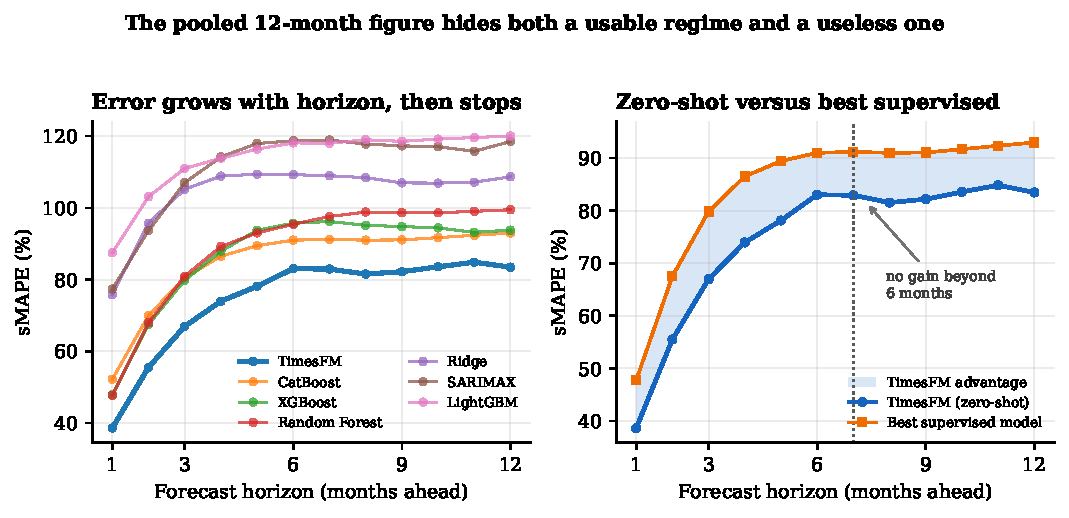
\includegraphics[width=\textwidth]{fig9_horizon.pdf}
\caption{Forecast error by horizon step, averaged over the eight cities. Left: all seven
models. Right: the zero-shot model against the best supervised model at each step, with
the shaded area showing the advantage and the dotted line marking where error stops
growing. Per-city comparison at the pooled horizon is given in the supplementary material.}
\label{fig:horizon}
\end{figure}

\subsection{The ranking depends on the metric}

sMAPE, MAE and RMSE select the same model in only four of the eight cities
(Figure~\ref{fig:disagreement}). In Belo Horizonte and Bras\'ilia each of the three names
a different winner. By MAE, TimesFM ranks first in seven of eight cities; by RMSE it
leads in four, while LightGBM leads in two and Ridge in two despite ranking last and
second-to-last overall on the primary metric. A model can win on RMSE by being
conservative at epidemic peaks while being poor everywhere else. Reporting a single
metric would have concealed this, and would have produced a different conclusion.

\begin{figure}[htbp]
\centering
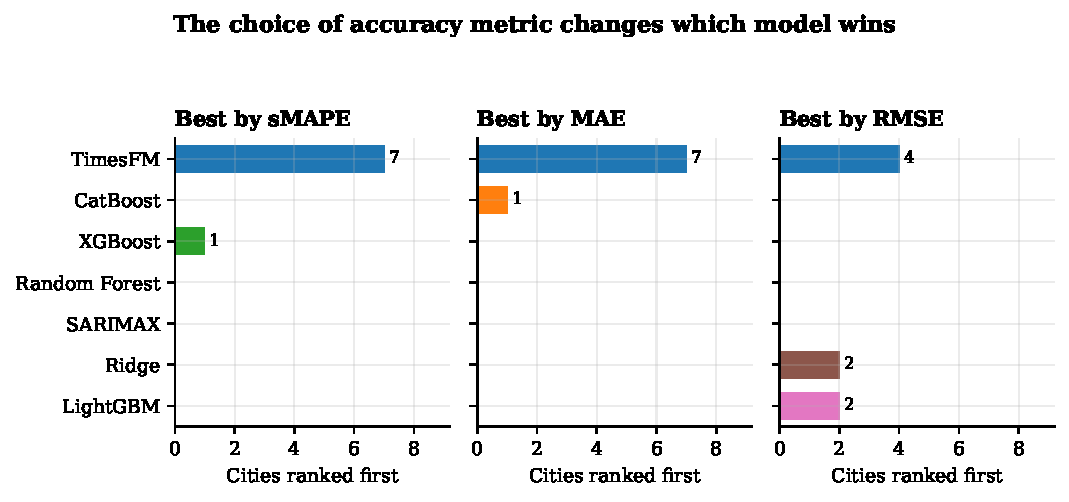
\includegraphics[width=\textwidth]{fig4_metric_disagreement.pdf}
\caption{Number of cities in which each model ranks first, under each of the three
accuracy metrics. The ranking is stable under sMAPE and MAE and fragments under RMSE.}
\label{fig:disagreement}
\end{figure}

\subsection{Intervals are calibrated, except when it matters}

Conformal calibration works in aggregate: at the nominal 95\% level empirical coverage was
91.9\% for TimesFM under the multiplicative construction and 93.0\% under the additive
one, and 91.0\% and 91.4\% for CatBoost. Coverage degrades mildly with horizon, from
95.8\% at one month to 91.7\% at twelve.

The failure is temporal. Restricted to the years before 2024, coverage at the nominal 95\%
level is 92.8\% (multiplicative) and 93.6\% (additive). In 2024 it falls to 87.2\% and
69.2\% respectively (Figure~\ref{fig:calibration}). Sharpness is poor throughout: the
median 95\% interval spans 13.0 times the median observed count under the additive
construction and 25.8 times under the multiplicative one. Intervals are therefore honest
about ordinary variation and silent about the event a surveillance system most needs
warning of. The ranking of models by weighted interval score also reverses between the two
constructions, so no probabilistic ranking is claimed.

The operational reading is uncomfortable. A band that holds 93.6\% of the time across a
decade of ordinary years, and then admits only 69.2\% of observations during the one
epidemic in the series, would have given a health authority exactly the wrong impression
of its own reliability at the moment the forecast was being used to decide something. An
interval that is correct on average but conditionally wrong when the outcome is extreme
does not support the decision it would be consulted for.

\begin{figure}[htbp]
\centering
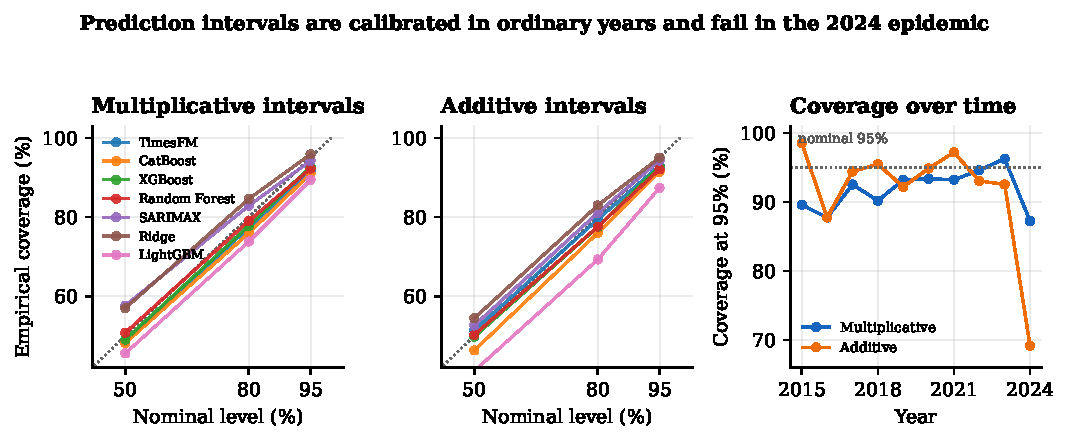
\includegraphics[width=\textwidth]{fig6_calibration.pdf}
\caption{Calibration of the conformal prediction intervals. Left and centre: empirical
coverage against nominal level under the two constructions; the dotted diagonal is perfect
calibration. Right: coverage at the nominal 95\% level by calendar year, showing the
collapse in 2024.}
\label{fig:calibration}
\end{figure}

\subsection{Combining models does not rescue the ranking}

The best of four combinations failed to beat the best single model of that city in seven
of eight cities (Table~\ref{tab:ensembles}). The exception is S\~ao Paulo, where the
median ensemble improves on the best member by 1.3 sMAPE points; elsewhere the shortfall
reaches 12.7 points in Rio de Janeiro. The median ensemble is the best combination at
79.0\% mean sMAPE, ahead of every individual model except TimesFM, because it resists
members that diverge. The metric dependence reappears and reverses the conclusion: on
sMAPE and MAE the best approach overall is a single model, TimesFM, while on RMSE it is
the stacked ensemble at 10{,}532 against 10{,}862.

% gerado por scripts/build_paper_assets.py -- nao editar a mao
\begin{table}[htbp]
\centering
\small
\caption{Individual models and model combinations on the same evaluation set, averaged
over the eight cities.}
\label{tab:ensembles}
\begin{tabular}{lrrrc}
\toprule
Approach & sMAPE (\%) & MAE & RMSE & Cities ranked first \\
\midrule
TimesFM & 74.9 & 3,082 & 10,862 & 5/8 \\
Median ensemble$\dagger$ & 79.0 & 3,392 & 10,908 & 1/8 \\
CatBoost & 83.4 & 3,691 & 11,165 & 1/8 \\
Inverse-error weighted ensemble$\dagger$ & 83.8 & 3,531 & 10,809 & 0/8 \\
XGBoost & 84.5 & 4,230 & 12,511 & 1/8 \\
Random Forest & 86.9 & 4,224 & 11,827 & 0/8 \\
Mean ensemble$\dagger$ & 87.6 & 3,787 & 10,979 & 0/8 \\
Stacked ensemble (Ridge)$\dagger$ & 94.8 & 3,526 & 10,532 & 0/8 \\
Ridge & 100.1 & 3,696 & 10,856 & 0/8 \\
SARIMAX & 108.6 & 4,070 & 11,531 & 0/8 \\
LightGBM & 116.2 & 5,435 & 11,874 & 0/8 \\
\bottomrule
\end{tabular}

\vspace{0.5em}
\begin{minipage}{\textwidth}
\footnotesize
$\dagger$ marks a combination of the seven individual models. Weights and the stacking
meta-model are fitted only on folds earlier than the one being predicted, so the
combination never sees the fold it is evaluated on. Individual models and combinations are
scored on exactly the same rows: the first 20 folds are withheld as a training window for
the combiners, leaving 1{,}188 predictions per approach per city. Comparing a combination
evaluated on 99 folds against a single model evaluated on 119 would favour the combination,
because the withheld folds are those with the shortest training window.
\end{minipage}
\end{table}


% =============================================================================
\section{Discussion}

A foundation model applied with no local training matched or exceeded six purpose-trained
models at a 12-month horizon, ranking first by sMAPE and by MAE in seven of eight cities.
The comparison is asymmetric in its disfavour: the supervised models were refitted on each
city at each of 119 folds, while TimesFM saw the series only as context at inference. The
operational consequence is about cost rather than accuracy, since a single unmodified
model removes the per-city selection and retraining that a national programme would
otherwise carry.

Three results bound that conclusion, and we consider them the more useful contribution.
The model ranking depends on which accuracy metric is chosen in half the cities. Interval
coverage collapses during the one epidemic in the series. And combining models does not
help. Together these argue against deploying any single model on the strength of a
benchmark.

That verdict converges with independent evidence. The 2024 Dengue Forecasting Sprint,
prospective and at state level with climate covariates, concluded that no model excelled
consistently and that ensembles were needed for stability \citep{Araujo2026sprint}. Two
evaluations with opposite designs reaching the same place is stronger than either alone.
Where we differ is on the remedy: their members were six independent teams with different
feature sets, ours are seven models sharing one lag structure and no covariates.
Aggregation rewards disagreement between members, and by construction we removed most of
it, so our negative result concerns combining redundant models rather than ensembles in
general. \citet{Silva2026capitals} covered all 27 capitals at four-week horizons with
covariates, and a reader choosing a model for short-term warning should prefer that work;
\citet{Freitas2025bands} produced probabilistic bands at finer spatial resolution, from
the posterior of one specified model rather than by auditing coverage across several.

Several limitations bound these conclusions. The outcome is notified cases, so what is
forecast is the behaviour of the surveillance system rather than biological incidence. No
exogenous covariates were used, and the TimesFM advantage may narrow once supervised
models receive informative features a zero-shot model cannot consume. Validation is
internal and temporal, not external. Hyperparameters were fixed rather than tuned, which
mirrors low-maintenance deployment but understates a tuned pipeline. One checkpoint was
evaluated on eight capitals, and smaller municipalities with shorter histories are
untested. We did not attempt any remedy for the 2024 distribution shift, although
training-set augmentation with synthetic extremes \citep{Bannoud2026augment} and adaptive
conformal methods \citep{Gibbs2021adaptive} are the obvious candidates. Bootstrap
intervals resample serially dependent predictions and are reported as a lower bound.

Evaluating foundation models as a low-maintenance forecasting layer within InfoDengue is
supported by these results, particularly for municipalities where a bespoke model is not
feasible. Reading their output as outbreak warning is not.

% =============================================================================
\section*{Declarations}

\paragraph{Data and code availability.} Monthly case data are publicly available through
the InfoDengue API (\url{https://info.dengue.mat.br/api/}). All analysis code, processed
data, result files and the scripts that generate every table and figure are available at
\url{https://github.com/fabianofilho/dengue-time-series}.

\paragraph{Funding.} No external funding was received.

\paragraph{Conflicts of interest.} The authors declare no conflicts of interest.

\paragraph{Author contributions.} Following the CRediT taxonomy.
\textbf{Fabiano Barcellos-Filho:} Conceptualization, Data curation, Formal analysis,
Investigation, Methodology, Project administration, Software, Validation, Visualization,
Writing: original draft, Writing: review and editing.
\textbf{Jos\'e Trajano:} Conceptualization, Formal analysis, Methodology, Supervision,
Writing: review and editing.
\textbf{Wilson Falco:} Data curation, Investigation, Software,
Writing: review and editing.
All authors read and approved the final manuscript.

\paragraph{Declaration of the use of generative AI and AI-assisted technologies in the
writing process.} During the preparation of this work the authors used a large language
model based assistant to support literature organisation, drafting, and the generation of
analysis and figure code. After using this tool the authors reviewed and edited the
content as needed, verified every reported number against the underlying analysis output,
and take full responsibility for the content of the publication. The tool is not an author
and does not meet authorship criteria.

\paragraph{Supplementary material.} Descriptive statistics of the eight series, absolute
error by model and city, the per-city metric comparison, full interval calibration by
model and construction, and five additional figures are provided as a supplementary PDF.

\paragraph{Acknowledgements.} Surveillance data were obtained from InfoDengue
(Fiocruz/FGV). TimesFM was developed by Google DeepMind.

% =============================================================================
\bibliographystyle{plainnat}
\bibliography{refs/references}

\end{document}
